\section{Magnetooptischer Kerr-Effekt}

\subsection{Theoretische Grundlagen}

  \subsubsection{Magnetisierung von Materie}

  Äußere Magnetfelder $\vec{H}$ verusachen in Materie eine materialabhängige makroskopische Magnetisierung $\vec{M}$.
  In dia- ($\chi_V<0$) und paramagnetischen ($\chi_V>0$) Materialien lässt sich dieser Zusammenhang mit der Vakuumpermeabilität $\mu_0$ durch
  \begin{equation}
    \mu_0 \vec{M} = \chi_V \vec{B}_0}
  \end{equation}
  beschreiben.
  Die Magnetisierung hängt also über $\chi_V$ linear von der äußeren magnetischen Flussdichte $\vec{B}_0= \mu_0 \vec{H}$ ab.

  In ferromagnetischen Materialien hingegen bleibt nach Abschalten des äußeren Magnetfeldes eine Magnetisierung zurück, die zu der in \cref{fig_magnetismen} abgebildeten Hysteresekurve führt.

  \begin{figure}[H]
      \centering
      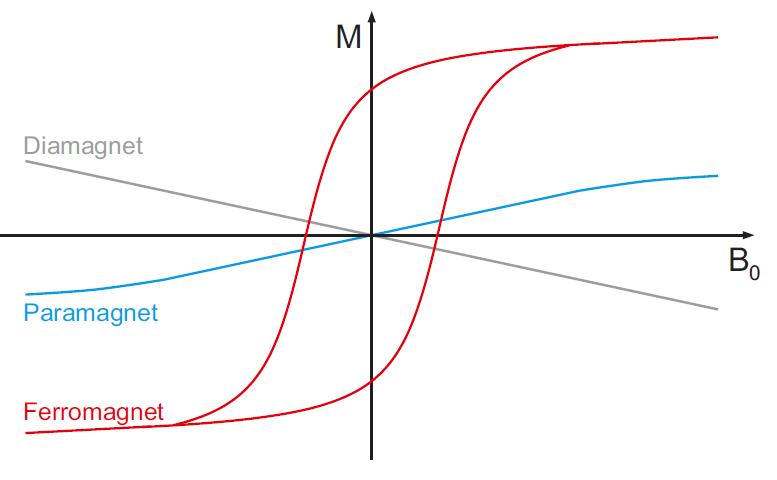
\includegraphics[width=0.8\textwidth]{img/magnetismen}
      \caption{Schematische Abhängigkeit der Magnetisierung $M$ dia-, para- und ferromagnetischer Materialien vom angelegten äußeren Magnetfeld $B$. \cite{anleitung}
      \label{fig_magnetismen}
  \end{figure}

  %den Kram mit den Domänen lasse ich jetzt weg, weils irgendwie weitgehend egal ist.

  \subsubsection{Polarisation und Materie}
  Die Wechselwirkung von elektromagnetischen Wellen mit Materie kann über den Brechungsindex
	\begin{align*}
		\tilde{n} = n + ik
	\end{align*}
  beschrieben werden, wobei $n$ die Brechung und $k$ die Absorption beschreibt.
  Hieraus kann Reflektion und Transmission berechnet werden.
  Das Hinzufügen eines externen magnetischen Feldes verursacht wie beschrieben eine Magnetisierung in Abhängigkeit von den magnetischen Eigenschaften der Materie.
  Dadurch ändert sich auch der Brechungsindex je nach Polarisation der einfallenden elektromagnetischen Welle.

  Linear polarisiertes Licht kann als Überlagerung einer rechts- und einer linkszirkular polarisierten elektromagnetischen Welle beschrieben werden.
  Beim Treffen auf Materie werden diese Teilwellen mit unterschiedlicher Intensität und Phase reflektiert bzw. transmittiert.
	Im Ergebnis ist die Überlagerung der Wellen nicht mehr linear, sondern elliptisch polarisiert.
	Die Winkeldifferenz zwischen Hauptachse der Ellipse und der Polarisationsrichtung des initialen linear polarisierten Lichts ist die Rotation und die Änderung der Intensität die Exzentrizität.

  Diese Rotation wird im Falle von Transmission Faraday-Rotation und im Falle von Reflektion Kerr-Rotation mit dem Kerr-Winkel $\theta_K$ genannt.

  In Ferromagneten liegen stets unterschiedlich magnetisierte Domänen (weissche Bezirke) vor.
  Da jedoch bei Messungen des Kerr-Winkels viele Domänen belichtet werden, wird ein mittlerer Kerr-Winkel gemessen, der als proportional zur Magnetisierung angenommen werden kann.

\subsection{Aufbau & Durchführung}

  \begin{figure}[H]
      \centering
      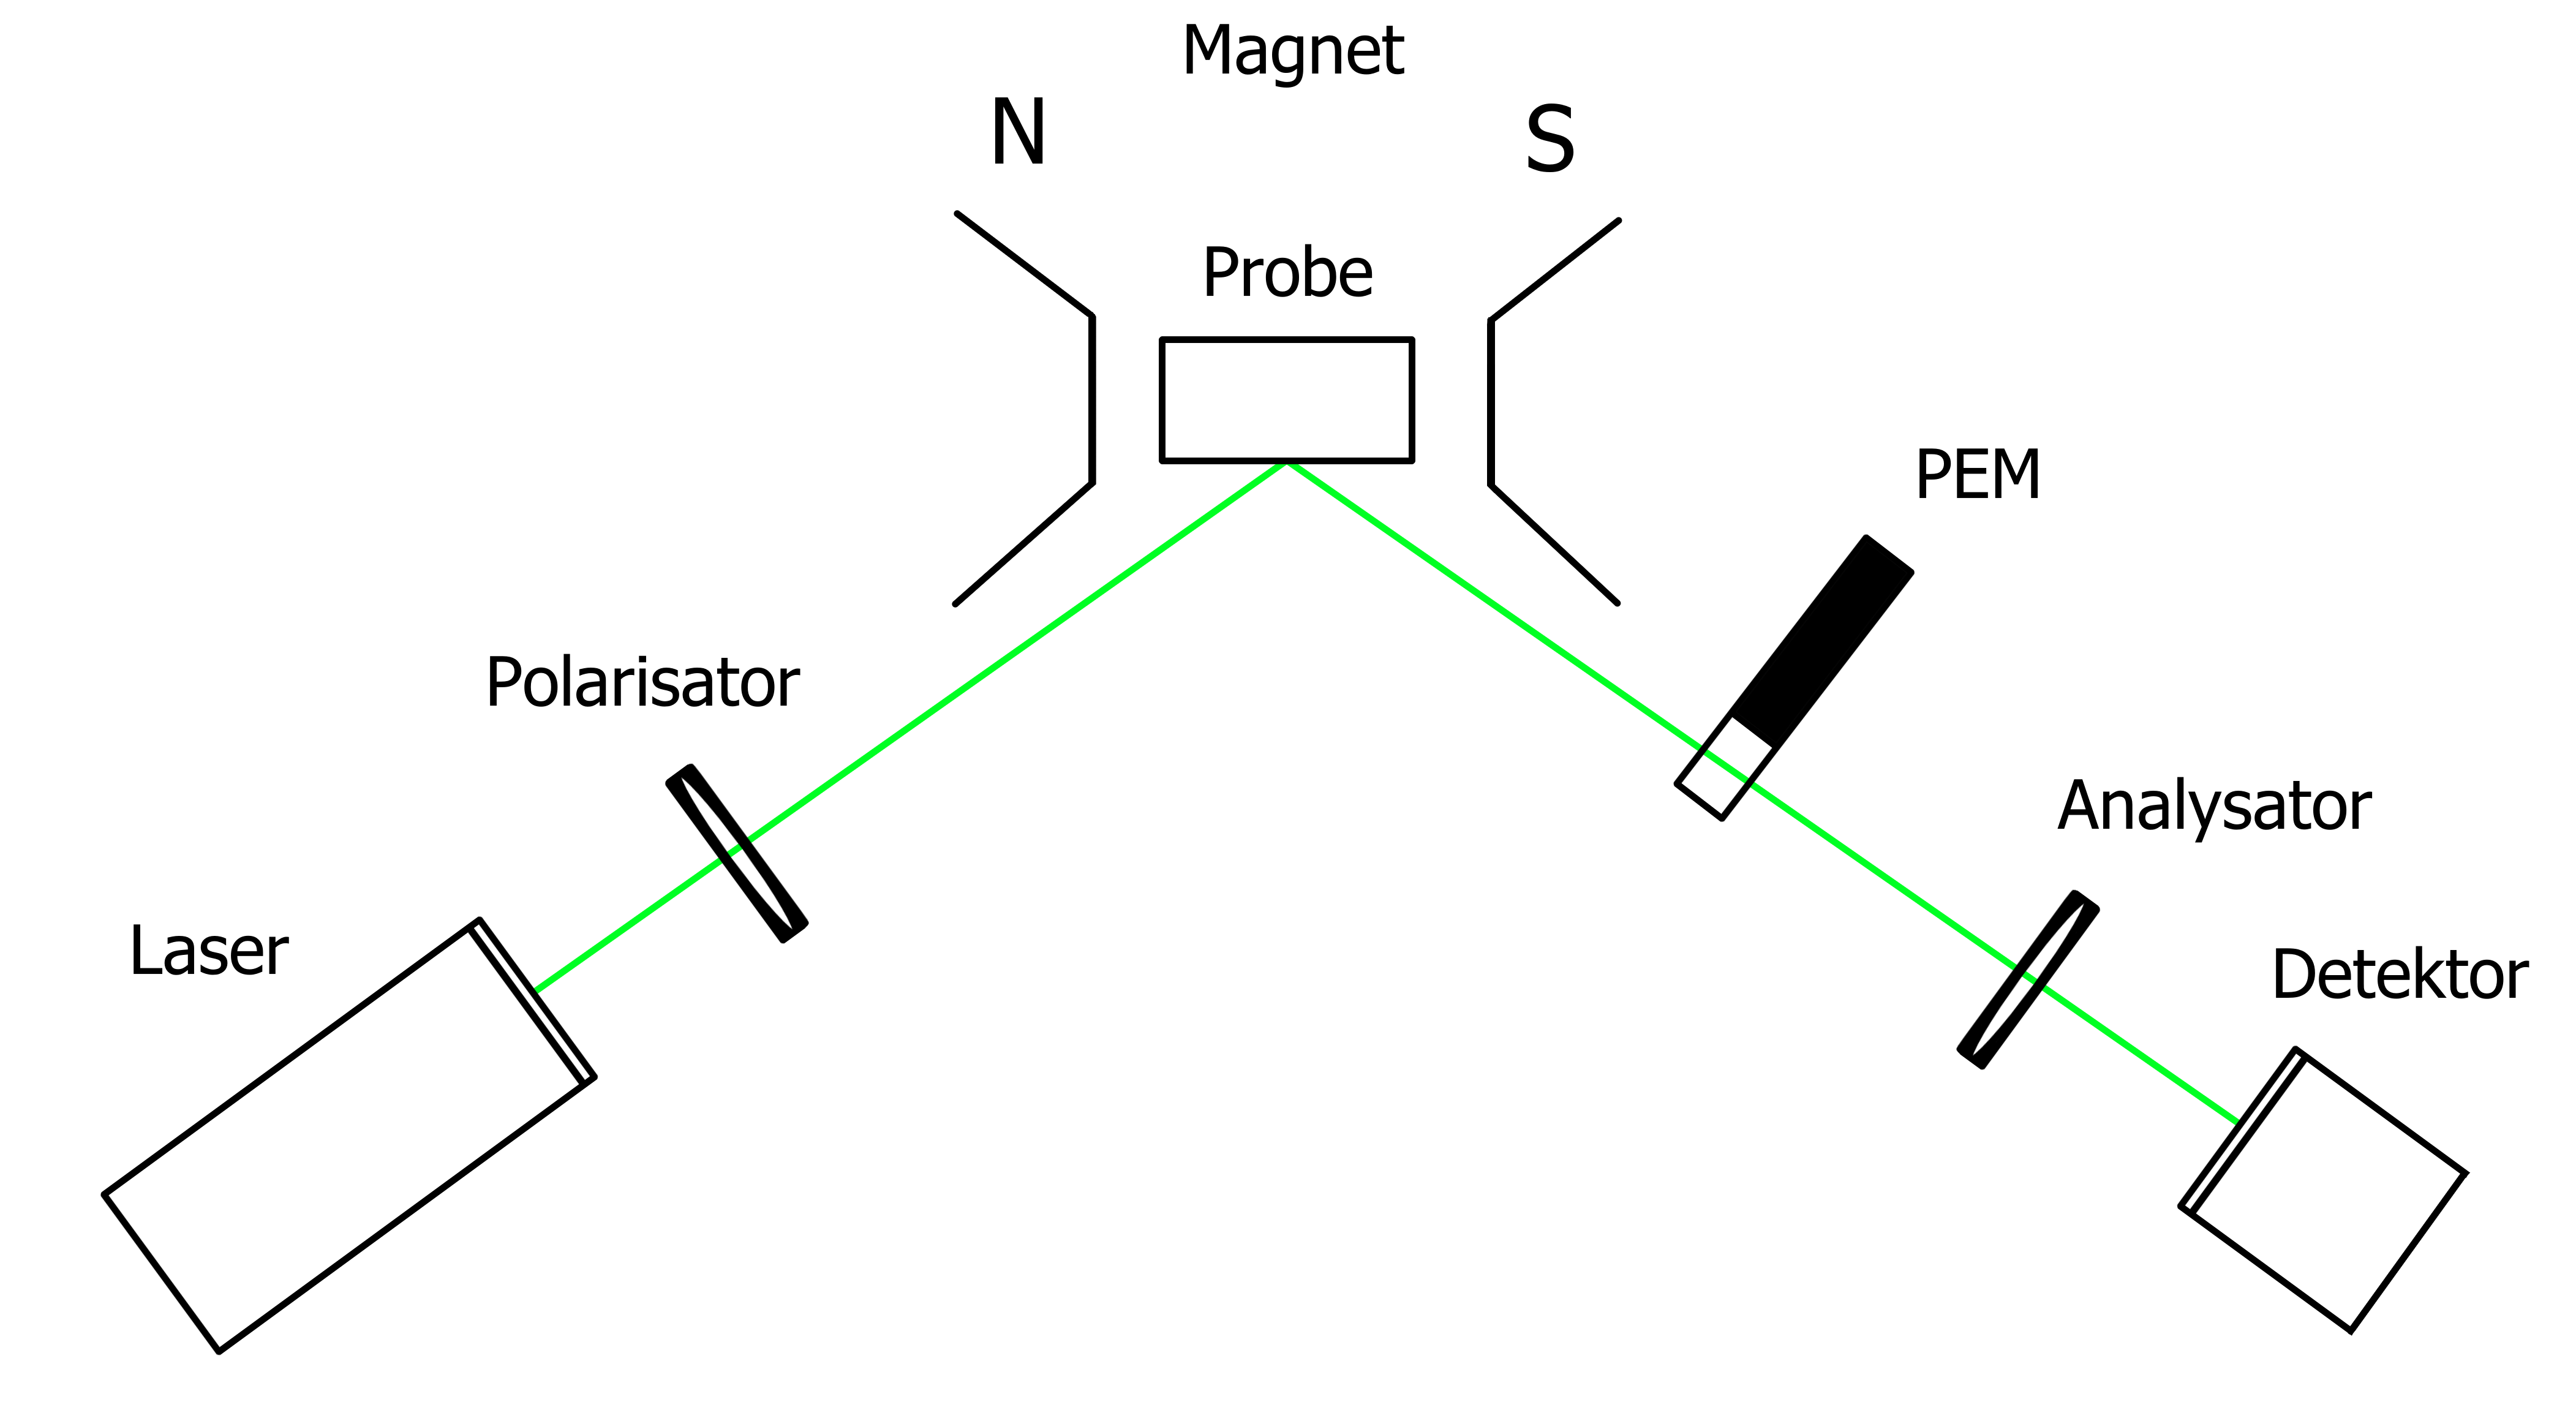
\includegraphics[width=0.8\textwidth]{img/setup2}
      \caption{Schematische Darstellung des experimentellen Aufbaus zur Messung der Magnetisierung in Abhängigkeit vom äußeren Magnetfeld.
      \label{fig_magnetismen}
  \end{figure}


\subsection{Ergebnisse & Diskussion}

%Letzter Tag Hysterese Kurve mit moke.
%Glenn-Thompson-Prisma für Polarisator und Analysator. PEM für Modulation + Lock-In-Verstärker für besseres Signal
%CoPt ist nur Out of plane Magnetisierbar. Der CrO2 nur in plane. Die jeweils anderen nur kurz gemessen, um das festzustellen.
